%%%%%%%%%%%%%%%%%%%%%%%%%%%%%%%%%%%%%%%%%%%%%%%%%%%%%%%%%%%%%%%%%%%%%%%%%%%%%%%%
%%                           ONDER DE LOEP ARTIKEL                            %%
%%%%%%%%%%%%%%%%%%%%%%%%%%%%%%%%%%%%%%%%%%%%%%%%%%%%%%%%%%%%%%%%%%%%%%%%%%%%%%%%

\artikelfoto{Variabelen in de eerste graad}{}{Filip Moons \\ Katrin Klingbeil}{img/loep/letters.jpg}

\startcontents[inhoudloep]

\begin{multicols}{2}
	
	\inhoudstafelloep			% om inhoudstafel voor het loep artikel te tonen

% TODO : tikz/end/ fouten, Alexander: is mij niet direct duidelijk waar het zit... de figuren komen er goed uit, dus gewoon zo laten lijkt mij

\section{Inleiding}
De introductie van letters in het wiskundeonderwijs markeert de overgang van rekenkunde naar algebra en valt in de meeste landen samen met de stap van het basisonderwijs naar het secundair onderwijs en dat is in Vlaanderen niet anders. Toch verloopt die overgang zelden probleemloos: veel leerlingen hebben moeite om te begrijpen wat variabelen precies voorstellen. Omdat variabelen al snel overal in de wiskundeles opduiken, kan zo’n gebrekkig begrip verstrekkende gevolgen hebben.

In deze loep nemen we je uitgebreid mee in de moeilijkheden die kunnen ontstaan bij de begripsvorming van leerlingen rond variabelen en hoe je hier in de klas mee om kunt gaan. We geven een grondig wiskundedidactisch overzicht en veel informatie over de overgang van wiskunde in de lagere school naar die in het secundair onderwijs. 

We starten met een stukje geschiedenis, om te laten zien dat het huidige letterrekenen pas zo’n 400 jaar bestaat in de vorm waarin we het vandaag onderwijzen. Dat noopt meteen tot enige nederigheid. Als het al eeuwen duurde voordat de mensheid het letterrekenen onder de knie had, is het niet verrassend dat veel leerlingen hier ook mee worstelen.

Daarna behandelen we de verschillende rollen die variabelen kunnen spelen. Dit sluit mooi aan bij het onderstaande minimumdoel:

\begin{kader}{Minimumdoel 1e graad A-stroom wiskunde}{} 6.11 De leerlingen gebruiken letters als onbekenden, als variabelen en voor veralgemeningen.
\end{kader}

In deze loep gebruiken we, in lijn met de internationale onderzoeksliteratuur, iets andere termen. Zo worden in deze loep de termen \textit{letters} en \textit{variabelen} door elkaar gebruikt, waarbij ze als synoniemen worden beschouwd. De rol van letters als variabelen in het minimumdoel komt overeen met die van een \textit{veranderlijke grootheid}, terwijl de rol van letters voor veralgemeningen overeenkomt met het \textit{veralgemeend getal}.

Vervolgens gaan we in op de veranderende betekenis van het gelijkheidsteken en op misconcepties over de betekenis van variabelen. Deze thematiek de aanleiding voor deze loep. Beide auteurs voerden een grootschalig onderzoek uit bij 2220 Duitse 12- tot 14-jarigen (vergelijkbaar met leerlingen in onze eerste graad) en hun 103 leerkrachten, naar hoe misconcepties rond variabelen zich na een maand algebraonderwijs doorheen de tijd ontwikkelen, onlangs gepubliceerd in \textit{Educational Studies in Mathematics} (Klingbeil \& Moons, 2025). Katrin Klingbeil is lerarenopleider wiskunde aan de Universiteit Duisburg-Essen en promoveert er in de algebradidactiek. Filip Moons is universitair docent in de wiskundedidactiek aan het Freudenthal Instituut van de Universiteit Utrecht. 

Deze loep zal voor leerkrachten wiskunde, zeker die in de eerste graad A-stroom, zeer herkenbaar zijn. Veel van wat hier theoretisch onderbouwd wordt, hebben zij ongetwijfeld al bij je leerlingen opgemerkt. Door deze observaties te kaderen en het bestaande wetenschappelijk onderzoek op een toegankelijke manier te delen, hopen we je een dieper inzicht te bieden in hoe hardnekkig bepaalde misconcepties kunnen zijn en hoe specifieke didactische keuzes begripsvorming kunnen bevorderen of juist belemmeren. Daarnaast hopen we duidelijk te laten zien dat resultaten van vakdidactisch onderzoek een meerwaarde kunnen zijn voor het lesgeven. Ook voor leerkrachten in de tweede en derde graad is dit relevant, want misconcepties rond variabelen verdwijnen zelden vanzelf, sommige moeilijkheden blijven hardnekkig en kunnen daardoor het verdere wiskunde-leren beïnvloeden. Bovendien geven we ook voorbeelden uit latere jaren.

Tot slot: in Uitwiskeling verschenen er reeds loeps rond algebraonderwijs, weliswaar met een iets andere insteek. Zowel `\textit{Algebralessen met applets}' (24/1) als `\textit{Algebra oefenen met inzicht}' (29/1) blijven ook nog vandaag bijzonder relevant en vormen een mooie aanvulling op dit verhaal.

In elk geval: veel lees- en lesgeefplezier!

\section{Een beetje geschiedenis}
Eén van de oudste problemen waarin `variabelen' voorkomen stamt uit het Oude Egypte (ongeveer 3000 v.\,Chr.), waar volgende taak opduikt op de Rhind-paprys:
\begin{quote}
``Een stuk land moet verdeeld worden onder twee erfgenamen op zo’n manier dat de ene vier keer zoveel krijgt als de andere. Hoe?''
\end{quote}
Als het land bijvoorbeeld 15 eenheden telde, losten de Oude-Egyptische wiskundigen dit op met iets wat wij vandaag een woordformule zouden noemen: ``\textit{Een hoeveelheid en haar kwart tellen samen op tot 15.}'' Om de vergelijking op te lossen, vertrokken ze van een \textit{valse assumptie} (Přibyl et al., 2018). Zo gokten ze bijvoorbeeld dat de hoeveelheid 4 was; telden daar een kwart bij en kwamen zo op 5. Vervolgens zagen ze dat dit getal met 3 vermenigvuldigd moest worden om op 15 te komen. Daarom vermenigvuldigden ze ook hun gok (4) met 3, wat 12 opleverde als oplossing. Tot slot controleerden ze dat 12, samen met zijn kwart, inderdaad 15 geeft.
\afbeelding[7cm]{img/loep/rhind.png}{Probleem 26 op de Rhind-papyrus (Chace et al., 1929)}{rhind}

De oude Egyptenaren hadden dus al, via woordformules, een notie van het concept `variabele'. Daarmee konden ze de vergelijking verbaal weergeven, zonder dat ze met deze variabele rekenden bij het oplossen van de vergelijking. De ontwikkeling om die variabelen te gaan noteren met letters, begint rond 300 v.\,Chr. bij Euclides. In zijn beroemde werk \textit{Elementen} gebruikte hij letters om onbepaalde grootheden weer te geven, zoals lengtes van lijnstukken, oppervlaktes of hoekgroottes. Het idee dat je met deze letters ook rekenkundige bewerkingen kon uitvoeren, ontbrak echter nog bij Euclides. Dan is het lange tijd stil. Pas in de 13e eeuw, introduceert Nemorarius het gebruik van hoofdletters voor variabelen. Doordat bewerkingen in die tijd nog niet consistent genoteerd werden, weten we wel dat hij bewerkingen met letters uitvoerde, maar is het niet altijd duidelijk wat hij precies deed.  Een belangrijke stap volgde in de 15e eeuw bij de zogenaamde ‘Cossisten’, die een variabelensymbool `cosa' gebruikten -- wat stond voor `iets' of een ´ding' -- in combinatie met een gestandaardiseerde manier van werken met machten. Met Vieta’s werk in 1591 werd het mogelijk om formules te schrijven met hoofdletters voor variabelen en een duidelijkere notatie voor bewerkingen. Hij onderscheidde zelfs onbekende grootheden (die hij noteerde met klinkers) van bekende grootheden (die hij met medeklinkers aanduidde). Descartes bracht in 1637 verdere vernieuwing door kleine letters aan het einde van het alfabet zoals $x$, $y$ en $z$ te introduceren voor onbekenden, samen met symbolen voor machten, haakjes en wortels. Ten slotte introduceerde Leibniz in 1676 het gebruik van letters met indices zoals $x_1,x_2,\ldots,x_n$ waardoor de algebraïsche notatie ontstond die nog steeds de basis vormt van hoe we variabelen en formules vandaag opschrijven.

Tot slot: voor wie zich afvraagt waarom de letter $x$ alomtegenwoordig is om een onbekende aan te duiden: dat komt uit de Arabische wereld. In Arabische, wiskundige teksten werd vaak het woord \emph{šay’} (shay'), wat gewoon `het ding' betekent, gebruikt voor de onbekende. Toen deze teksten via de Moren het middeleeuwse Spanje bereikte, werden ze naar het Latijn vertaald. Daar werd \emph{šay’} in eerste instante weergegeven met het Griekse symbool $\chi$ (uitgesproken als \emph{chi}). Dat klonk voor de Spanjaarden als een harde \emph{ch}, en in de latere Latijnse vertalingen werd het uiteindelijk vereenvoudigd tot de letter $x$. De echte reden waarom we vandaag nog altijd vaak $x$ gebruiken in algebralessen, is dus dat de Spanjaarden geen \textit{chi} kunnen uitspreken. Een fijn filmpje hierover van Terry Moore vind je als TED talk op YouTube (zie bronnen).


\section{De verschillende rollen van variabelen}
Eén van de belangrijkste zaken om te onthouden na het lezen van deze loep is dat een variabele in de wiskunde van de eerste en tweede graad van het secundair onderwijs altijd een \textbf{verwijzing naar een kwantiteit} is. Pas later kunnen variabelen ook meer abstracte wiskundige objecten voorstellen zoals bijvorbeeld een matrix of stochast.

Daarnaast vormt het feit dat letters zoals $x$, $y$ of $b$ verschillende rollen kunnen spelen één van de meest onderschatte moeilijkheden voor leerlingen. Merk op dat Vieta in 1591 deze rollen al deels gebruikte en er zelfs zijn notatie op afstemde. In de vakliteratuur worden doorgaans vijf rollen onderscheiden die variabelen kunnen aannemen in het wiskundeonderwijs (Arcavi et al., 2017).

\begin{kader}{Onthoud}{Variabele = Verwijzing naar een kwantiteit}
Variabelen verwijzen (initieel) \textbf{altijd naar een kwantiteit (`hoeveelheid')}. Zo'n kwantiteit kan een \textbf{getal} zijn (een element uit een getallenverzameling) of een \textbf{maat} (een getal met een eenheid).\end{kader}
\subsection{Plaatshouder}
Bij een variabele als plaatshouder kan de variabele worden gezien als een ‘lege doos’ waarin specifieke waarden kunnen worden ingevuld. Zie \autoref{plaatshouder} voor een typische oefening waarbij de variabelen $a$ en $b$ de rol van plaatshouder spelen.
\afbeelding{img/loep/plaatshouder.jpg}{Variabelen als plaatshouder (VBTL 2)}{plaatshouder}

\subsection{Onbekende}
De variabele als onbekende komen we tegen bij vergelijkingen, ongelijkheden en stelsels. In de vergelijking $2x + 5 = 7$ stelt de variabele $x$ een onbekende waarde voor. De rol van variabelen als onbekende draait eigenlijk om het zoeken naar ‘waarmakers’ in de getallenverzameling waarop de vergelijking werkt. Zo'n waarmaker kan worden bepaald door rekenregels toe te passen.
\afbeelding{img/loep/vlekoefening.jpg}{Vlekoefeningen, hierbij zijn de vlekken variabelen als onbekenden}{vlek}

De rol van variabelen als onbekenden is leerlingen in de eerste graad al bekend vanuit het lager onderwijs. Zogenaamde ‘vlekoefeningen’ (zie \autoref{vlek}) zijn oefeningen waarbij leerlingen getallen moeten invullen op de plaats van de vlek. Dat gebeurt intuïtief, zonder gebruik van expliciete methodes om vergelijkingen op te lossen en zonder de variabelen als letters te noteren. Het is ook vaak de enige rol van variabelen die leerlingen vanuit het basisonderwijs kennen.

Merk ook op dat het allereerste spoor van letterrekenen in de geschiedenis, ‘Een kwantiteit en zijn kwart tellen op tot 15’, eigenlijk de variabele (de ‘kwantiteit’) als onbekende betreft, wat wij nu noteren als de $x$ in de vergelijking $x + \frac{x}{4} = 15.$
\subsection{Veranderlijke grootheid}
Bij een functie wordt de waarde van de ene variabele, de uitvoervariabele (de afhankelijke variabele, in de wiskundeles meestal $y$), bepaald door de waarde van de andere, de invoervariabele (onafhankelijke variabele, meestal $x$). In dit geval spelen beide variabelen de rol van veranderlijke grootheid. In een functie met functievoorschrift $y = 2x + 3$ kun je de waarde van $y$ berekenen door een concrete waarde toe te kennen aan $x$. Zo geldt bijvoorbeeld: als $x=4$, dan is $y=11$.
\afbeelding{img/loep/invoeruitvoer.jpg}{Invoer-uitvoermachine}{veranderlijke}

Merk op dat dit een heel andere rol is dan die van de variabele als plaatshouder: de waarde van $y$ is hier geen ‘lege doos’, maar hangt expliciet af van de waarde van $x$. Bovendien zijn $x$ en $y$ hier geen onbekenden: je kunt de waarde van $x$ niet afleiden door een waarmaker te zoeken.

\subsection{Veralgemeend getal}
In \autoref{gegeneraliseerd} drukken we met de variabelen $a$ en $b$ uit dat voor alle getallen geldt dat het kwadraat van de som van twee getallen, gelijk is aan de som der kwadraten van deze getallen plus tweemaal hun product. We beschrijven dus een algemeen patroon. De variabelen $a$ en $b$ nemen zo de rol aan van een veralgemeend getal. De variabele is een `algemeen' getal waarvan de waarde niet gegeven is, of initieel eigenlijk niet van belang is: het moet `alle' getallen als waarde kunnen aannemen terwijl de bewerking waar blijft.
\afbeelding{img/loep/gegeneraliseerd.png}{Variabelen als veralgemeende getallen}{gegeneraliseerd}
\end{multicols}
\afbeelding[12cm]{img/kipfunctie.jpg}{}{}
\begin{multicols}{2}
\subsection{Parameter}
Een variabele kan ook de rol van parameter aannemen. In de uitdrukking $y = c\cdot x$, is $c$ een parameter. Het is een vaste waarde, de evenredigheidsfactor, die ervoor zorgt dat we oneindig veel recht-evenredige verbanden tegelijkertijd kunnen beschrijven. De letter $c$ is geen onbekende wiens waarde je moet zoeken, ook geen invoervariabele die telkens verandert. Parameters noemen we ook weleens `slapende' variabelen of `veranderlijke constanten'. Ze stellen ons onder meer in staat om bijvoorbeeld alle kwadratische functies te definiëren: $f(x)=a\cdot x^2+b\cdot x+c$. Door $a,\;b$ en $c$ een concrete waarde te geven (met $a\not = 0$), kunnen we alle mogelijke kwadratische functies beschrijven. Merk op dat de rol van $a, b$ en $c$ totaal verschillend is van $x$ en $f(x)$, die hier veranderlijke grootheden zijn. 

\end{multicols}
\begin{testjezelf}{Welke rol speelt de variabele?}
\section*{Vraag 1}
In het handboek `Van Basis Tot Limiet 2' (Leerboek Getallenleer/Algebra, Data en Onzekerheid) vinden we volgende oefening:
\begin{center}
    \includegraphics[scale=1]{img/loep/rol1.png}
\end{center}
\begin{vraagenantwoord}

\vraag{Wat is de rol van $A$ en $r$ voordat we een concrete waarde voor $r$ invullen?}
 \antwoord{\textbf{Veranderlijke grootheid}: het invoeren van om het even welke waarde voor $r$, levert een waarde op voor de uitvoervariabele $A$, die in dit geval de oppervlakte geeft van een bol met straal $r$.}
 \vraag{Wat is de rol van $A$ en $r$ als we $r$ willen vervangen door 4 cm?}
 \antwoord{In dit geval wordt $r$ een \textbf{plaatshouder} van 4 cm, de rol van $A$ is een \textbf{onbekende} geworden: we moeten nog wat rekenen om tot de waarde 188,50 cm$^2$ te komen. Toch is de rol hier minder afgelijnd: je kan met evenveel stelligheid zeggen dat $A$ en $r$ nog steeds \textbf{veranderlijke grootheden} zijn, maar dat $r$ als invoervariabele nu even een concrete waarde aanneemt.}
 \end{vraagenantwoord}

\section*{Vraag 2}
In het Nederlandse VWO-examen Wiskunde B (vergelijkbaar met onze Wiskunde 6u) werd in 2022 de onderstaande vraag gesteld over de inverse van $y=\ln{x}$. Ook al ligt de leerstof buiten bereik van de eerste graad, toch is de volgende vraag interessant: kun jij achterhalen welke rol de variabele $p$ in de verschillende onderdelen speelt? Een lijn wordt in Vlaanderen trouwens een `rechte’ genoemd. Let op: de nummering van de vragen kan voor ons Vlamingen wat verwarrend zijn, vandaar de hulplijntjes. Het is niet nodig om de examenvragen op te lossen, bepaal enkel de rol van de letter $p$ in elke vraag (overgenomen uit Drijvers, 2025).
\begin{center}
    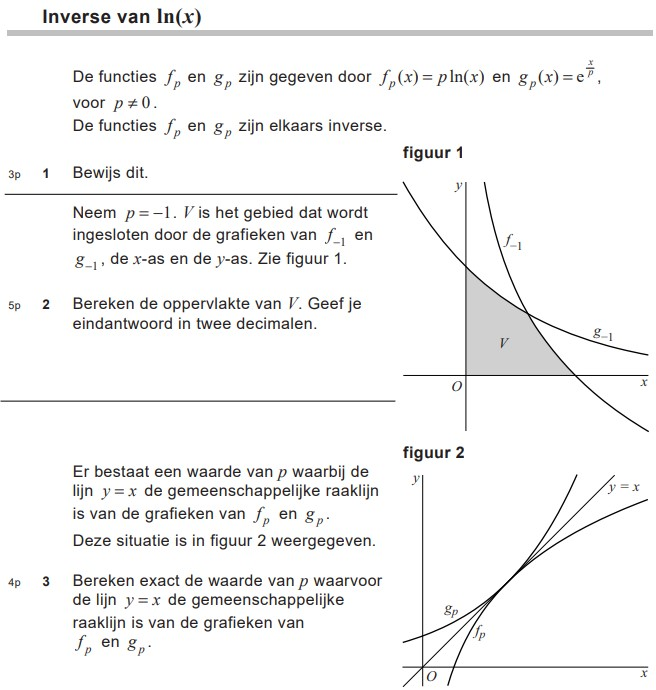
\includegraphics[scale=0.7]{img/loep/wiskundeBlijnen.jpg}
\end{center}

\begin{vraagenantwoord}
    
 \vraag{Wat is de rol van $p$ in vraag 1?}
 
 \antwoord{\textbf{Veralgemeend getal}: we bewijzen dat voor alle mogelijke waarden van $p$, $f_p$ en $g_p$ elkaars inverse functie zijn. We beschrijven een algemeen patroon, het hele punt van de vraag is net dat de exacte waarde van $p$ hier eigenlijk niet van belang is. Sommige lezers zullen allicht ook \textbf{parameter} antwoorden. Dat is zeker het geval in het deel voor vraag 1: met $p$ beschrijven we inderdaad alle mogelijke functies $f_p$ en $g_p$.}
 \vraag{Wat is de rol van $p$ in vraag 2?}
 
 \antwoord{\textbf{Parameter}: door het kiezen van een exacte getalwaarde voor $p$ (namelijk $p=-1$), beschrijven we de functies $f_{-1}$ en $g_{-1}$. De letter $p$ kan hier ook als \textbf{plaatshouder} worden gezien. }
  \vraag{Wat is de rol van $p$ in vraag 3?}
 
 \antwoord{\textbf{Onbekende}: we gaan op zoek naar een exacte getalwaarde $p$ die ervoor zorgt dat de rechte $y=x$ de gemeenschappelijke raaklijn is.}

\end{vraagenantwoord}

\end{testjezelf}
\begin{multicols}{2}

\subsection{Gevolgen voor de klaspraktijk}
Zoals je in de kader ‘Test jezelf: Welke rol speelt de variabele?’ hebt ervaren, is de rol van variabelen fluïde: eenzelfde variabele kan tijdens een wiskundig vraagstuk meerdere keren van rol wisselen. Het is bovendien geen exacte wetenschap: soms kun je discussiëren over welke rol een variabele op dat moment precies vervult. Toch is dat niet de kernboodschap van dit deel. Want ook al kunnen variabelen impliciet van rol veranderen tijdens een oefening, en ook al is het herkennen van die rollen nooit een doel op zich, voor leerlingen die voor het eerst met variabelen kennismaken, blijft de betekenis van variabelen vaak een mysterie. Het speelt zeker een rol in het taalgebruik: zo spreken we niet over de onbekende van een functie of de veranderlijke grootheid in een vergelijking. Maar veel explicieter worden die verschillende rollen zelden gemaakt, waardoor leerlingen zelf moeten ontdekken dat variabelen in verschillende contexten een andere rol kunnen opnemen. Onderzoek toont aan dat dit het begrip van variabelen aanzienlijk kan bemoeilijken (Usiskin, 1988). 

Specifiek in Vlaanderen hebben we daarbij een vrij unieke leerlijn rond de introductie van variabelen. Zonder expliciet over letterrekenen te spreken, komen leerlingen in de meeste handboeken al variabelen tegen als veralgemeende getallen bij het leren van rekenregels in de verschillende getalverzamelingen. Vrij snel daarna maken ze kennis met variabelen als onbekenden bij het oplossen van eerstegraadsvergelijkingen in $\mathbb{Z}$. Dit is een prima gelegenheid om expliciet te maken dat de letters een andere rol spelen dan bij de rekenregels van getalverzamelingen. In het tweede middelbaar worden variabelen pas apart bestudeerd bij het formeel aanleren van de rekenregels van het letterrekenen, waarbij opnieuw de rol van veralgemeende getallen wordt aangenomen. De eerste graad eindigt meestal met een hoofdstuk over recht- en omgekeerd evenredig waarin variabelen opnieuw verschijnen, nu voor het eerst als veranderlijke grootheden. De evenredigheidsfactor daarentegen speelt de rol van parameter. Parallel aan deze leerlijn duiken ook formules op in de meetkunde, zoals voor oppervlakte en omtrek, waar variabelen opnieuw als veranderlijke grootheden fungeren. 

In de tweede en derde graad keren alle rollen van variabelen geregeld terug: als veranderlijke grootheden in de functieleer, als onbekenden bij uiteenlopende soorten vergelijkingen, en als parameters bij het beschrijven van functiefamilies. In de derde graad wordt het variabelenbegrip bovendien verder opgerekt: in de statistiek verschijnen kansvariabelen met een bepaalde verdeling, in de algebra worden matrices met variabelen genoteerd, en in de analyse kunnen onbekenden zelfs functies voorstellen in het kader van differentiaalvergelijkingen. Voor veel leerlingen is het begrip tegen die tijd voldoende gerijpt, zodat het schakelen tussen de verschillende rollen doorgaans geen problemen meer oplevert.

Terug naar de eerste graad: de eerste kennismaking met letters is meestal de commutativiteit in $\mathbb{N}$, waarbij variabelen voor het eerst opduiken als veralgemeende getallen in $\forall a, b \in \mathbb{N}: a + b = b + a$. Dankzij de (her)introductie van verzamelingenleer in de eerste graad weten leerlingen vaak wel dat $a$ en $b$ willekeurige elementen zijn uit de verzameling van natuurlijke getallen. Toch kan dit voor sommige leerlingen nog te abstract zijn: reacties als `\textit{Maar we kunnen toch niet weten wat $a$ en $b$ zijn?}’ zijn heel normaal bij leerlingen die voor het eerst met variabelen als veralgemeende getallen geconfronteerd worden en zijn voor de leraar een aanleiding om de betekenis op scherp te stellen. De leerlingen kunnen het gevoel hebben dat de `oefening' $a + b$ niet af is, omdat er geen concreet antwoord volgt. Dit fenomeen staat in de literatuur bekend als de \textit{lack of closure} (Kieran, 1992). Het is dus uitermate belangrijk om mee te geven dat de formule niet aangeeft wat de uitkomst is van de optelling, maar wel dat de optellingen uit beide leden altijd dezelfde uitkomst geven.

Er zijn twee goede praktijken om hiermee om te gaan: het gebruik van woordformules en het expliciet benoemen van de rol die variabelen spelen wanneer nieuwe rollen voor het eerst opduiken.

\subsubsection{Woordformules}
Het is aan te raden om langere tijd \textit{woordformules} te gebruiken, eventueel naast het formele gebruik van variabelen. Zo kun je $\forall a, b \in \mathbb{N}: a + b = b + a$ ook verwoorden als: `\textit{Als }\texttt{getal\_a}\textit{ en }\texttt{getal\_b} \textit{ twee willekeurige natuurlijke getallen zijn, dan is} \texttt{getal\_a} + \texttt{getal\_b gelijk aan getal\_b} + \texttt{getal\_a}; \textit{met andere woorden: je mag getallen van volgorde wisselen bij het optellen van natuurlijke getallen.}' Door woordformules te gebruiken, geef je betekenis aan de wiskundige notatie en help je leerlingen om een brug te slaan tussen concrete taal en abstracte symbolen. Dit is bijzonder waardevol, omdat leerlingen van 12 jaar vaak nog nooit variabelen op deze manier hebben gezien, en woordformules kunnen helpen om die overgang vlotter te maken. Hoewel het voorbeeld hier wat abstract is, zijn woordformules in concrete contexten waarin de variabelen een duidelijke betekenis hebben, al helemaal zinvol. Zo is het zeker verstandig om bijvoorbeeld bij opperlvakteformules eerst de notatie vanuit het basisonderwijs te gebruiken, bijvoorbeeld voor een rechthoek: \textit{Oppervlakte = Lengte $\times$ Breedte}, pas later stap je over naar formules met uitsluitend letters.

\subsubsection{Rollen expliciet benoemen}
Daarnaast is het belangrijk om expliciet te zijn over de nieuwe rollen die variabelen kunnen aannemen wanneer die voor het eerst voorkomen. Het doel is niet dat leerlingen die rollen zelfstandig moeten herkennen, maar wel dat jij als leerkracht benoemt welke rollen al voorbij zijn gekomen en welke nieuwe rol er nu bijkomt. Zo kun je bij het introduceren van vergelijkingen even stilstaan bij het feit dat variabelen eerder al gebruikt zijn in rekenregels of oppervlakte- en omtrekformules (als veralgemeende getallen), en dat er nu de rol van onbekende bij komt, waarbij we op zoek gaan naar een specifieke waarde voor de variabele. Bij het behandelen van recht- en omgekeerd evenredig is het belangrijk om de invoer-uitvoerrelatie tussen $y$ en $x$ duidelijk te benoemen en uit te leggen dat dit opnieuw een andere rol van variabelen, die van veranderlijke grootheden, die verschilt van veralgemeende getallen: we drukken nu een samenspel tussen variabelen uit (meer bepaald een relatie tussen $y$ en $x$, $y$ wijzigt in functie van $x$) in plaats van een algemene regel waarin de variabelen los van elkaar staan (zoals de $a$ en $b$ in in  $(a+b)^2=a^2+2ab+b^2$) We noemen dit ook een covariatie.

Tot slot biedt de vakdidactische literatuur heel wat argumenten om de leerlijn rond variabelen anders op te bouwen dan we in Vlaanderen traditioneel gewend zijn. Verschillende onderzoeken wijzen erop dat het variabelebegrip vrij eng blijft wanneer het uitsluitend vanuit onbekenden of veralgemeende getallen wordt opgebouwd. Daarom pleiten diverse auteurs ervoor om variabelen van meet af aan in de context van functies te introduceren. Arcavi (1994) benadrukt dat functies een krachtige omgeving vormen om het idee van variabelen te ontwikkelen, omdat leerlingen variabelen daar meteen leren zien als veranderlijke grootheden die met elkaar in relatie staan. Vanuit zo’n functionele benadering duiken andere rollen vanzelf op: in een rechtevenredig verband wil men in een concrete context bijvoorbeeld weten welke $x$-waarde overeenkomt met een bepaalde $y$-waarde, waardoor de rol van onbekende wordt geïntroduceerd; de evenredigheidsfactor fungeert daarbij als parameter, enzovoort.

Een ideale manier om de kracht van variabelen aan leerlingen te laten zien, is de noodzaak ervan introduceren aan de hand van een goocheltruc. Door de goocheltruc met de leerlingen te doorlopen, creëer je haast spontaan de nood om te laten zien dat de truc altijd werkt, waarbij variabelen haast vanzelf om de hoek komen loeren. Naast de goocheltruc in de volgende lesactiviteit, vind je nog veel meer trucs in de loep `\textit{Goochelen in de wiskundeles}' (28/2).
\end{multicols}
\begin{lesactiviteit}{Variabelen introduceren met goocheltrucs}
Schrijf ergens het getal 7 op een kaartje en stop het in een toverhoed of verstop het in de boekentas van een leerling. Laat de leerlingen volgende stappen uitvoeren en vraag hen hun berekening op te schrijven op een kladblaadje.\begin{multicols}{2}
\setlength\itemsep{-0.5em} 
\begin{enumerate}

	
	\item Kies een getal,
	\item Tel er 8 bij op,
	\item Vermenigvuldig het resultaat met 3,
	\item Trek er 4 vanaf,
	\item Tel je gekozen getal erbij,
	\item Deel door 4,
	\item Tel er 2 bij op,
	\item Trek er het gekozen getal vanaf.
\end{enumerate}
\end{multicols} 
\noindent Als alle leerlingen goed geteld hebben, komen ze op 7 uit.\\

Doorloop dit zo nodig tweemaal, waarbij leerlingen twee verschillende getallen mogen kiezen. Laat ze nadien de uitdrukking zelf abstraheren waarbij ze gewoon in hun berekeningen hun gekozen getal door \textit{getal} (woordformule) of $x$ (abstracte afleiding) moeten vervangen. Het is geen slecht idee dat in zo'n eerste fase ook in de 8 stapjes te doen van de truc.

\begin{minipage}[t]{0.25\textwidth}
\textbf{Concreet voorbeeld}\\
17 = gekozen getal
\begin{enumerate}\setlength\itemsep{-0.4em}
  \item $17$
  \item $17 + 8 = 25$
  \item $25 \cdot 3 = 75$
  \item $75 - 4$ = 71
  \item $71 + 17 = 88$
  \item $88/4 = 22$
  \item $22 + 2 = 24$
  \item $24 - 17 = \textbf{7}$
\end{enumerate}
\end{minipage}\hfill
\begin{minipage}[t]{0.40\textwidth}
\textbf{Woordformule}\\
getal = gekozen getal
\begin{enumerate}\setlength\itemsep{-0.4em}
  \item $\text{\small getal}$
  \item $\text{\small getal}+8$
  \item $(\text{\small getal}+8)\cdot 3 = 3\cdot\text{\small getal} + 24$
  \item $3\cdot \text{\small getal}+24-4 = 3\cdot\text{\small getal}+20$
  \item $3\cdot\text{\small getal}+20+\text{\small getal} = 4\cdot\text{\small getal}+ 20$
  \item $(4\cdot\text{\small getal}+20)/4 = \text{\small getal} + 5$
  \item $\text{\small getal} + 5 + 2 = \text{\small getal} + 7$
  \item $\text{\small getal}+7-\text{\small getal} = \textbf{7}$
\end{enumerate}
\end{minipage}\hfill
\begin{minipage}[t]{0.27\textwidth}
\textbf{Abstracte afleiding}\\
$x =$ het gekozen getal
\begin{enumerate}\setlength\itemsep{-0.4em}
  \item $x$
  \item $x+8$
  \item $(x+8)\cdot 3 = 3x + 24$
  \item $3x+24-4 = 3x+20$
  \item $3x+20+x = 4x+ 20$
  \item $(4x+20)/4 = x + 5$
  \item $x + 5 + 2 = x + 7$
  \item $x+7-x = \textbf{7}$
\end{enumerate}
\end{minipage}

\textbf{\textit{Varianten}}\\
\noindent Dit is meteen een stevig voorbeeld. Je kunt ook andere varianten bedenken waarbij jij het getal kan raden dat de leerling uitkomt, los van het getal waarmee de leerling vertrokken is. Bijna altijd komt het neer op het gekozen getal ergens terug af te trekken of weg te delen (bv. neem een getal, verdubbel het, vermenigvuldig het resultaat met 5, deel het resultaat door je gekozen getal, je bekomt altijd 10). Het is ook heel fijn om leerlingen zelf zo'n truc te laten bedenken of zelfs als toetsvraag leerlingen zo'n trucje te laten bewijzen.!

\end{lesactiviteit}
\begin{multicols}{2}

\section{De veranderende rol van het gelijkheidsteken}
Stel je even voor dat je als 12-jarige de onderstaande uitdrukkingen ziet: 
\begin{vraagenantwoord}
\vraag{$5\cdot3=\ldots$}
\vraag{$7\cdot\ldots=21$}
\vraag{$8+1=\ldots$}
\vraag{$f(x)=2x+4$}
\end{vraagenantwoord}

Wat valt op? Vraag 4 kun je helemaal niet uitrekenen, en juist dat kan erg lastig zijn voor leerlingen die de overstap maken van de lagere school naar het middelbaar onderwijs. Heel impliciet lijkt namelijk de rol van het gelijkheidsteken te veranderen. In de lagere school (vragen 1 tot en met 3) koppelen leerlingen het gelijkheidsteken vaak automatisch aan een oproep om iets uit te rekenen: zien ze een ``='', dan verwachten ze dat ze een berekening moeten uitvoeren die tot een uitkomst leidt. Terwijl de echte betekenis van het gelijkheidsteken is dat beide leden dezelfde waarde hebben.

Deze veranderende rol is goed te begrijpen vanuit de wiskundedidactische theorie van de proces-objectdualiteit (Sfard, 1991). Die stelt dat je een wiskundige uitdrukking zoals ``2 + 3'' op twee manieren kunt zien: als een proces, namelijk het optellen van 2 en 3, of als een object, namelijk de som zelf. In het lager onderwijs lijkt het gelijkheidsteken vooral het begin van een rekenproces, terwijl het eigenlijk aangeeft dat twee objecten gelijk in waarde zijn. Om ``2 + 3 = 5'' goed te begrijpen, moeten leerlingen inzien dat zowel ``2 + 3'' als ``5'' objecten zijn die dezelfde waarde vertegenwoordigen,  en dat het gelijkheidsteken niet het begin van een rekenproces aanduidt, maar juist de gelijkheid van die twee objecten uitdrukt. 

De proces-objectdualiteit speelt niet alleen bij het gelijkheidsteken, maar komt terug in vrijwel elk wiskundig concept. Denk bijvoorbeeld aan functies: aanvankelijk ervaren leerlingen een functie vooral als een proces, zoals uitrekenen van functiewaarden of nulpunten berekenen, maar naarmate ze vooruitgaan in hun wiskundige ontwikkeling, moeten ze functies ook leren zien als objecten op zich, bijvoorbeeld om het concept van de afgeleide functie goed te kunnen begrijpen.

Bovendien gebruiken leraren in de lagere school het gelijkheidsteken soms verkeerd, bijvoorbeeld om tussenstappen die niet gelijk zijn toch aaneen te rijgen. Zo kan bij de som $76+23$ het getal $23$ worden gesplitst in $20+3$, wat dan fout genoteerd wordt als $=76+20=96+3=99$. Dit misbruik van het gelijkheidsteken, ook wel \textit{breien} genoemd, komt wereldwijd voor (Capraro et al., 2011). In de nieuwe minimumdoelen voor het basisonderwijs wordt dit nu tegengegaan: in het vierde leerjaar is een correct gebruik en interpretatie van het gelijkheidsteken expliciet opgenomen als doelstelling (Onderwijsdoelen, 2025).

\section{Misconcepties over de betekenis van letters}
Een misconceptie is een foutief conceptueel schema dat leerlingen houvast geeft, maar niet in overeenstemming is met de juiste wiskundige ideeën. In dit hoofdstuk bespreken we de meest frequente misconcepties die kunnen voorkomen rond de betekenis van variabelen. Deze misconcepties hebben één gemene deler: variabelen worden soms (tijdelijk) niet gezien als verwijzingen naar kwantiteiten. Om straks helemaal mee te zijn, loont het de moeite om eerst de test hieronder door te nemen. Ze vormt de rode draad waarnaar we verderop vaak zullen verwijzen.

\end{multicols}
\begin{testjezelf}{SMART-test `Betekenis van letters'}
\noindent
\begin{minipage}[c]{0.25\linewidth}
    \includegraphics[width=\linewidth]{img/loep/qr.png} 
\end{minipage}%
\hspace{0.05\linewidth}%
\begin{minipage}[c]{0.7\linewidth}
Als je de QR-code scant, kom je terecht bij de digitale versie van de SMART-test \textit{Betekenis van letters}. Deze test bevat 6 vragen die peilen naar een correct begrip van variabelen. De test werd ontwikkeld binnen het SMART-project (``Specific Mathematics Assessments that Reveal Thinking''), dat in 2008 startte aan de Universiteit van Melbourne (Australië). Dit project heeft als doel om wetenschappelijk gevalideerde, diagnostische toetsen te ontwikkelen die nagaan in hoeverre leerlingen conceptueel inzicht hebben of misconcepties vertonen over verschillende wiskundige inhouden. Het doel van deze toetsen is leraren een duidelijk beeld geven van de denkfouten in hun klas waardoor ze hun lessen hierop afstemmen (Steinle et al., 2009).\end{minipage}\\
\includegraphics[width=\linewidth]{img/loep/smart_dutch3.pdf}

Klingbeil et al.\ (2023) voerden bijkomende validaties uit met leerlingeninterviews bovenop het Australische werk. Daaruit bleek dat deze 6 meerkeuzevragen op zich voldoende sterke aanwijzingen geven voor het bestaan van bepaalde misconcepties. De kleuren en afkortingen naast de afleiders, worden later toegelicht. Het correcte antwoord staat altijd als eerste, dat is natuurlijk niet het geval bij de digitale versie die aan leerlingen wordt aangeboden.
\end{testjezelf}
\begin{multicols}{2}
\subsection{Letter-als-Object (LO)}
De Letter-als-Object (LO) misconceptie treedt op wanneer een variabele wordt gezien als een naam voor een object of als het object zelf (Küchemann, 1981). Zo interpreteren sommige leerlingen in de \includegraphics[scale=0.04]{img/loep/duck.png} Eendenvraag de $e$ in de vergelijking $6e=12$ als \colorbox{kleurmeestalLO}{\textit{eend}} of \colorbox{kleurmeestalLO}{\textit{eenden}}. De variabele wordt dan opgevat als een ding, in plaats van als een verwijzing naar een kwantiteit — in dit geval de prijs van een eend. Je hebt dit fenomeen ongetwijfeld zelf al in de klas meegemaakt. Vaak gaat het samen met een beperkt begrip van het gelijkheidsteken: een uitspraak als ``6 eenden is gelijk aan 12 euro'' lijkt logisch, maar verhult dat de linker- en rechterzijde verschillende grootheden uitdrukken en dus nooit werkelijk gelijk kunnen zijn.

\subsubsection{Het student-professorenprobleem}
Een wereldberoemd probleem dat te maken heeft met het correct interpreteren van het gelijkheidsteken en de Letter-als-Object misconceptie is het \textit{student-professorenprobleem}. Neem een kladblaadje en een pen, lees het probleem hieronder en probeer het binnen 20 seconden op te lossen (en laat het zeker ook eens door je leerlingen proberen):

\begin{kader}{Student-professorenprobleem}{}
Schrijf een vergelijking op met de variabelen $S$ en $P$ die de volgende uitspraak weergeeft: ``\textit{Er zijn zes keer zoveel studenten als professoren op deze universiteit.}'' Gebruik $S$ voor het aantal studenten en $P$ voor het aantal professoren.
\end{kader}
Heb je toevallig $6S=P$ opgeschreven? Dan ben je zeker niet de enige! Verschillende onderzoeken (Clement, 1982; Kaput, 1985; MacGregor \& Stacey, 1993; Cohen \& Kanim, 2005; Soneira et al., 2018; Jankvist \& Niss, 2021) tonen aan dat een meerderheid van de deelnemers deze \textit{omkeerfout} maakt. Het correcte antwoord is immers $6P=S$.

Er zijn twee belangrijke oorzaken voor de omkeerfout $6S=P$. De meest voorkomende is dat mensen de zin \textit{syntactisch vertalen} : ``zes keer ($6$) zoveel studenten ($S$) als ($=$) professoren ($P$)'', waardoor de structuur van de zin rechtstreeks maar foutief wordt overgenomen in de vergelijking. Een andere oorzaak noemen we de \textit{statistische vergelijking}: mensen stellen zich bijvoorbeeld een lokaal voor met zes studenten ($=6S$) tegenover één professor ($=P$).
\end{multicols}
\afbeelding[10cm]{img/eend.jpg}{}{}
\clearpage
\begin{multicols}{2}
Welke redenering er ook achter zit, deze foute interpretatie wijst vaak op een verkeerd begrip van het gelijkheidsteken of op de Letter-als-Object-misconceptie: respondenten interpreteren de variabelen $S$ en $P$ als student(en) en professor(en), en niet als het \textit{aantal} studenten en het \textit{aantal} professoren. Wie variabelen én het gelijkheidsteken correct betekenis geeft, ziet in dat $6S=P$, oftewel ``zes keer het aantal studenten is gelijk aan het aantal professoren'', niet kan kloppen. Merk op dat de correcte betekenis van $S$ en $P$ letterlijk in de opgave stond.
\subsubsection{Letter-als-Eenheid (LE)}
De Letter-als-Eenheid (LE) misconceptie treedt op als variabele wordt gezien als de afkorting van een eenheid (Ball et al., 2001; Akhtar \& Steinle, 2017). Leerlingen die in de \includegraphics[scale=0.04]{img/loep/duck.png} Eendenvraag het antwoord \colorbox{randomkleurvanFilip}{\textit{euro}} geven, interpreteren de $e$ in de vergelijking $6e=12$ als de eenheid, namelijk euro's. Deze misconceptie kan voortkomen uit de lagere school, waarbij maateenheden zoals $m$ of $cl$ ook letters waren die in de wiskundeles opdoken voor meter en centiliter. Merk op dat de Letter-als-Eenheid eigenlijk een subtype is van de Letter-als-Object misconceptie: ook een eenheid is immers een object. In de SMART-test wordt dit subtype echter wel afzonderlijk onderscheiden met eigen afleiders in de betekenisvragen.

\subsubsection{Oplossing-als-Coëfficiënt (OC)}
Een voorbeeld van de Oplossing-als-Coëfficiënt (OC) misconceptie zie je in de \includegraphics[scale=0.04]{img/loep/fiets.png} Fietsvraag: de optie \colorbox{kleurmeestalOC}{$35f+10d=100$} bevat namelijk een specifiek antwoord op het vraagstuk. 35 fietsen (= 70 wielen) plus 10 driewielers (= 30 wielen) leveren samen precies 100 wielen op. De Oplossing-als-Coëfficiënt-misconceptie ontstaat dus als de variabele wordt gezien als de afkorting van een object en de coëfficiënten als mogelijke oplossing (Küchemann, 1981). Leerlingen die OC-antwoorden geven, lossen intuïtief eerst het vraagstuk op zonder vergelijking. Met het bekomen antwoord, construeren ze dan een (foute) vergelijking die hun specifiek antwoord als coëfficienten bevat. Merk op dat OC opnieuw een subtype is van de Letter-als-Object misconceptie.
\begin{figure*}[t]
    \centering
    \includegraphics[width=\textwidth]{img/loep/Klassen_Dutch.pdf}
    \caption{Kansen op antwoordopties per latente groep}
    \label{fig:latent}
\end{figure*}


Zoals je aan de kleuren van de antwoordopties in het overzicht van de vragen van SMART-test hierboven kunt zien, is elke foute afleider een mogelijke indicator van een misconceptie. De test bestaat uit drie groepen van telkens twee vragen: \textit{betekenisvragen}, die rechtstreeks peilen naar de betekenis van een variabele in een bepaalde context; \textit{additieve vragen}, waarin een vergelijking wordt gevraagd waarin twee variabelen via de optelling verbonden zijn; en \textit{proportionele vragen}, waarin de variabelen op een proportionele manier verbonden zijn als varianten op het student-professorenprobleem. Vermits de test op twee tijdstippen bij dezelfde leerlingen werd afgenomen,  werd ook een B-variant ontwikkeld, waarin equivalente vragen maar met een andere contexten werden gesteld. De LO misconceptie was een afleider in alle mogelijke vragen, LE enkel in de betekenisvragen, OC zowel in de additieve als proportionele vragen.

\subsection{Prevalenties latente groep \& hun evoluties}
\subsubsection{Latente groepen}
In Klingbeil \& Moons (2025) werden 2220 Duitse leerlingen van 12 tot 14 jaar oud (vergelijkbaar met onze eerste graad) door hun leraar gevraagd om na één week algebrales de bovenstaande SMART-test af te leggen, en deze na vier weken algebrales opnieuw te maken. Daarmee wilden we een antwoord krijgen op de vraag: \textit{Hoe vaakt komt de LO misconceptie en zijn subtypes bij 12- tot 14-jarigen voor en is er vooruitgang merkbaar na 4 weken algebraonderwijs?} Naast deze onderzoeksvraag, zijn we in vervolgonderzoek ook geïnteresseerd welke invloed de leraar heeft op de ontwikkeling van deze misconcepties. 

Vervolgens werd op deze data een \textit{latente transitieanalyse} uitgevoerd. Zo’n latente transitieanalyse is een statistische methode die in de antwoordpatronen van leerlingen vooreerst groepen probeert te destilleren: twee leerlingen die het model in een groep plaatst, moeten op basis van hun antwoorden heel hard op elkaar lijken, twee leerlingen in verschillende latente groepen moeten zoveel mogelijk verschillen. Het zijn \textit{latente} groepen: je kan ze niet direct onderscheiden, het is een samenspel van antwoorden waaruit je patronen destilleert die een onderliggend denkbeeld verraden. Bepaalde combinaties van antwoorden geven immers inzicht in het begrip van leerlingen. Door dit zowel voor als na een lessenreeks algebra te bekijken, kun je bovendien nagaan hoe dit begrip in de loop van de tijd zich ontwikkelt: dat is een \textit{transisitieanalyse}.

Concreet konden we op beide tijdstippen vijf latente groepen onderscheiden, weergegeven in \autoref{fig:latent}. Deze figuur laat per latente groep zien wat de kans is om een bepaalde indicator te kiezen (correct of een specifieke misconceptie). We beschrijven de latente groepen kort en ordenen van minder naar meer correcte antwoorden:
\begin{figure*}[b!]
    \centering
    \includegraphics[width=\textwidth]{img/loep/alluviaal.png}
    \caption{Toestromingsdiagram van de latente groep voor- en na 4 weken algebraonderwijs.}
    \label{fig:alluviaal}
\end{figure*}
\begin{itemize}
\item \colorbox{kleurOCaddLOelders}{\textbf{OC in additieve vragen, LO elders}}\\
\noindent Deze groep valt op door een zeer grote kans (92\%) op een Oplossing-als-Coëfficiënt interpretatie bij additieve vragen, gecombineerd met een Letter-als-Object interpretatie bij de andere vragen. Deze leerlingen lijken systematisch letters als objecten te zien.
\item \colorbox{kleurmeestalOC}{\textbf{Meestal OC}}\\
\noindent Deze groep geeft Oplossing-als-Coëfficiënt antwoorden in zowel additieve als proportionele vragen, en kiest in betekenisvragen meestal voor een Letter-als-Object interpretatie.
\item \colorbox{kleurmeestalLO}{\textbf{Meestal LO, soms correct in additief}}\\
\noindent Deze groep vertoont een grote kans op een Letter-als-Object interpretatie, vooral bij proportionele en betekenisvragen. In additieve vragen is een correct antwoord ongeveer even waarschijnlijk als een LO-interpretatie. De OC-interpretatie komt in deze groep vrijwel niet voor.
\item \colorbox{kleurcorrectbetekenis}{\textbf{Correcte betekenis}}\\
\noindent Deze groep geeft meestal een correct antwoord wanneer er rechtstreeks naar de betekenis van variabelen wordt gevraagd. Zodra er echter bewerkingen met die variabelen nodig zijn, zoals in additieve en proportionele vragen, vallen ze toch terug op misconcepties: OC in additieve vragen, LO in proportionele vragen. Dit wijst op een ontluikende, maar nog oppervlakkige en onstabiele begripsvorming rond variabelen.
\item \colorbox{kleurmeestalcorrect}{\textbf{Meestal correct}}\\
\noindent Deze groep heeft een relatief hoge kans op een goed antwoord in bijna alle vraagtypes. Enkel bij proportionele vragen komt nog af en toe een LO-interpretatie voor. De OC-interpretatie is zo goed als afwezig.
\end{itemize}

Het valt op dat zelfs in de \textcolor{kleurmeestalcorrect}{$\blacksquare$} \textbf{Meestal correct}-groep de kans op een juist antwoord nog relatief beperkt blijft, en dat er geen aparte groep werd geïdentificeerd met vrijwel uitsluitend correcte antwoorden. Dit komt doordat er in de steekproef slechts 21 leerlingen waren (ongeveer 0,1\% van de totale steekproef) die op beide meetmomenten een volledig correcte test aflegden. Deze groep was te klein om door het statistische model als afzonderlijke latente groep herkend te worden. Daarnaast zien we dat de LE misconceptie relatief weinig voorkomt en er geen latente groepen gevonden werden die geïdentificeerd worden door een grote aanwezigheid van deze misconceptie.

\subsubsection{Initiële grootte en evoluties doorheen de tijd}
Dat brengt ons meteen tot de volgende kwestie: hoe groot zijn deze latente groepen initieel? En welke transities hebben leerlingen doorgemaakt na 4 weken algebraonderwijs? In \autoref{fig:alluviaal} zie je een zogeheten toestromingsdiagram dat al deze informatie weergeeft. In de transitiematrix van \autoref{tab:lta} vind je de grootte van de groepen op tijdstip 1 en 2 en de overgangspercentages die de overgangen weergeven tussen tijdstip 1 en tijdstip 2. Dit zijn de gekleurde lijnen in het toestromingsdiagram. 
Dat brengt ons meteen tot de volgende kwestie: hoe groot zijn deze latente groepen initieel? En welke transities hebben leerlingen doorgemaakt na 4 weken algebraonderwijs? In \autoref{fig:alluviaal} zie je een zogeheten toestromingsdiagram dat al deze informatie weergeeft. In de transitiematrix van \autoref{tab:lta} vind je de grootte van de groepen op tijdstip 1 en 2 en de overgangspercentages die de overgangen weergeven tussen tijdstip 1 en tijdstip 2. Dit zijn de gekleurde lijnen in het toestromingsdiagram. 
\begin{figure*}
\begin{tabel}
\renewcommand{\arraystretch}{1.2}
\begin{tabular}{m{6.cm}C{1.5cm}C{1.2cm}C{1.2cm}C{1.2cm}C{1.2cm}C{1.2cm}}
\hlinethick
\tableheader{Tijdstip 1} & \tableheader{Grootte T1} & \tableheader{1.} & \tableheader{2.} & \tableheader{3.} & \tableheader{4.} & \tableheader{5.} \\
\hlinethick
\colorbox{kleurOCaddLOelders}{\textbf{1.}} OC in additieve vragen, LO elders &\cellcolor{\rubriekkleur!50} 39,0\% & \textbf{58,2\%} & 0,0\% & 13,2\% & 18,6\% & 10,0\% \\
\colorbox{kleurmeestalOC}{\textbf{2.}} Meestal OC                     & \cellcolor{\rubriekkleur!50}10,9\% & 26,5\% & \textbf{37,6\%} & 12,4\% & 11,6\% & 11,9\% \\
\colorbox{kleurmeestalLO}{\textbf{3.}} Meestal LO, soms correct in additief & \cellcolor{\rubriekkleur!50}36,3\% & 9,5\% & 0,0\% & \textbf{68,6\%} & 1,7\% & 20,2\% \\
\colorbox{kleurcorrectbetekenis}{\textbf{4.}} Correcte betekenis        & \cellcolor{\rubriekkleur!50}6,6\%  & 34,7\% & 0,0\% & 6,3\% &\textbf{ 28,3\%} & 30,8\% \\
\colorbox{kleurmeestalcorrect}{\textbf{5.}} Meestal correct                  & \cellcolor{\rubriekkleur!50}7,2\%  & 10,5\% & 0,0\% & 6,4\% & 2,6\% &\textbf{ 80,5\%} \\ \hlinethick
\rowcolor{\rubriekkleur!50} \textbf{Grootte Tijdstip 2} &  & \textbf{32,1\%} & \textbf{4,1\%} & \textbf{32,3\%} & \textbf{11,2\%} & \textbf{20,3\%} \\
\hlinethick
\end{tabular}
\caption{Transitiematrix tussen tijdstip 1 en tijdstip 2}\label{tab:lta}
\end{tabel}

\end{figure*}
Er vallen een aantal tendenzen op:
\begin{itemize}
    \item In de meeste latente groepen, zijn de \textit{blijvers} (de diagonaal in de transitiematrix in \autoref{tab:lta}) de grootste groep: de meeste leerlingen verhuizen dus niet naar een andere latente groep na 4 weken algebraonderwijs. Enkel de leerlingen in \textcolor{kleurcorrectbetekenis}{$\blacksquare$} \textbf{Correcte betekenis} hebben een iets grotere kans (30,8\%) om over te schakelen op \\\textcolor{kleurmeestalcorrect}{$\blacksquare$} \textbf{Meestal correct}.
    \item Er zijn twee grote misconceptiegroepen: \textcolor{kleurOCaddLOelders}{$\blacksquare$} \textbf{OC in additieve vragen, LO elders} (39,0\% op tijdstip 1) en \textcolor{kleurmeestalLO}{$\blacksquare$} \textbf{Meestal LO, soms correct in additief} (36,3\% op tijdstip 1). Beide zakken naar iets meer dan 32\% op tijdstip 2, maar blijven groot. 
    \item De groep \textcolor{kleurmeestalOC}{$\blacksquare$} \textbf{Meestal OC} daalt van 10,9\% op tijdstip 1 naar 4,1\% op tijdstip 2. Opvallend: de groep ontvangt daarbij geen nieuwkomers. Enkel leerlingen die al in deze latente groep zaten, blijven er soms zitten. Er lijkt dus geen enkele didactische lesgeefstijl te zijn die deze latente groep groter maakt door invloed van de leerkracht.
    \item De grootste stijging zie je bij de groep \textcolor{kleurmeestalcorrect}{$\blacksquare$}{ \textbf{Meestal correct}}: deze groeit van 7,2\% naar 20,3\%. Dit is ook de meest stabiele groep: 80,5\% van de leerlingen blijft erin. 
    \item Kijk je naar de samenstelling van de groepen op tijdstip 2, dan zie je dat vooral \textcolor{kleurmeestalcorrect}{$\blacksquare$} \textbf{Meestal correct} en \textcolor{kleurcorrectbetekenis}{$\blacksquare$} \textbf{Correcte betekenis} veel `nieuwkomers' verwelkomen: respectievelijk 71,7\% en 83,2\%.
\end{itemize}
\subsection{Gevolgen voor de klaspraktijk}
Om ook het effect van de leraar zelf te bekijken, hebben we bij de 103 leraars individueel nagegaan hoeveel leerlingen in de loop van de lessenreeks zijn doorgeschoven naar groepen die beter scoorden, met name \textcolor{kleurcorrectbetekenis}{$\blacksquare$} \textbf{Correcte betekenis} en \textcolor{kleurmeestalcorrect}{$\blacksquare$}{\textbf{Meestal correct}}. Het resultaat: de verschillen tussen leraren bleken zeer groot. Gemiddeld schoof zo’n 31\% van de leerlingen door (Stand. Dev. = 22,5\%), maar bij tien leraren bleef dat onder de 5\% (waarvan twee zelfs vrijwel op 0\%), terwijl acht leraren boven de 75\% zaten en één leraar zelfs een vooruitgang van 90\% bereikte, dus zowat 9 op de 10 leerlingen verschoven in die klas naar een betere latente groep! Dit laat zien dat leraren sterk verschillen in hoe goed ze de begripsontwikkeling van hun leerlingen ondersteunen. Wel moeten we voorzichtig zijn: een deel van die verschillen kan ook te maken hebben met de samenstelling van hun klas. Onderstaand zie je twee toestromingsdiagrammen van twee klassen. 
    \afbeelding[8cm]{img/loep/teacher1_real_NL.png}{Toestomingsdiagram leraar 1}{}
    \afbeelding[8cm]{img/loep/teacher3_real_NL.png}{Toestromingsdiagram leraar 2}{}
Leraar 1 heeft initieel eigenlijk alle misconceptiegroepen in de klas: 45\%  van de leerlingen zit in \textcolor{kleurOCaddLOelders}{$\blacksquare$} \textbf{OC in additieve vragen, LO elders}, 19\% zit in \textcolor{kleurmeestalOC}{$\blacksquare$} \textbf{Meestal OC} en 34\% zit in \textcolor{kleurmeestalLO}{$\blacksquare$} \textbf{Meestal LO, soms correct in additief}. Na amper 4 weken algebraonderwijs zit 43\% van de leerlingen in \textcolor{kleurmeestalcorrect}{$\blacksquare$}{ \textbf{Meestal correct}} en 35\% \textcolor{kleurcorrectbetekenis}{$\blacksquare$} \textbf{Correcte betekenis}.

Een heel ander beeld zien we bij leraar 2: ook deze leerkracht heeft initieel 49\% van de leerlingen in \textcolor{kleurOCaddLOelders}{$\blacksquare$} \textbf{OC in additieve vragen, LO elders}, maar dit stijgt naar 54\% na 4 weken, waarbij de 6\% leerlingen in \textcolor{kleurcorrectbetekenis}{$\blacksquare$} \textbf{Correcte betekenis} ook naar deze misconceptiegroep verhuizen. Amper 1 op de 20 leerlingen zit na 4 weken in \textcolor{kleurmeestalcorrect}{$\blacksquare$}{ \textbf{Meestal correct}}, maar al die leerlingen zaten daar al vanaf het begin! Sommige leerlingen maken dus veel meer progressie afhankelijk van de leraar en sommigen gaan zelfs achteruit.

Als we de interviewdata bij dit onderzoek analyseren, wordt meteen duidelijk waarom. Wanneer leraren na vier weken nauwelijks vooruitgang of zelfs achteruitgang in begripsontwikkeling laten zien, gaat het vaak om degenen die zelden of nooit expliciet maken wat variabelen precies betekenen. Bovendien grijpen ze bovengemiddeld naar didactische trucjes die niets te maken hebben met de eigenlijke betekenis van variabelen. De bekendste truc, die in alle interviews opdook bij leraars die weinig progressie wisten te realiseren, is de \textit{fruitsaladealgebra}. Daarbij worden optellingen zoals $5a+2b-3a+b$ uitgelegd als: ``5 appels min 3 appels geeft 2 appels, 2 bananen plus 1 banaan geeft 3 bananen, dus $2a+3b$.''

Het probleem met dit soort uitleg is dat ze steunt op een foutieve objectinterpretatie van de variabelen $a$ en $b$. Het hoeft dan ook niet te verbazen dat leerlingen letters als objecten gaan zien, wanneer de leraar zelf dit verkeerde idee voortdurend benadrukt. Een betekenisvol alternatief om het optellen en aftrekken van lettervormen aan te brengen, wordt uitgewerkt in de vorm van een lesactiviteit.

Een andere veel voorkomende truc bij minder effectieve leraars is dat zij bij het oplossen van eerstegraadsvergelijkingen al snel grijpen naar oplossingsmethoden die draaien rond het ``naar de andere kant brengen'' van termen of factoren. Ook dat suggereert dat variabelen objecten zijn die je zelfs fysiek kan verplaatsen. Hoewel het idee van het wisselen van lid uiteraard een beoogde automatisatie is bij leerlingen, blijken leerkrachten die langere tijd de balansmethode hanteren — waarbij in het linker- en rechterlid telkens dezelfde bewerking wordt uitgevoerd — effectiever in het tegengaan van de Letter-als-Object-misconceptie.

Opvallend genoeg blijken de meest effectieve leraren juist degenen te zijn die steeds expliciet de betekenis van variabelen benadrukken en bevragen. Ze laten leerlingen langdurig en herhaald focussen op een correct begrip, bijvoorbeeld door hen die betekenis exact te laten opschrijven. Nadien controleren ze dit door concrete waarden in gegeven of opgestelde vergelijkingen te substitueren. Zo verdwijnen de meeste misconcepties gaandeweg.\end{multicols}
\afbeelding[9.7cm]{img/fruitalgebra.jpg}{}{}
\begin{lesactiviteit}{Hoe het optellen en aftrekken van lettervormen betekenisvol introduceren?}
Optellen en aftrekken met letters is in feite niets meer dan het consequent doortrekken van de rekenregels die leerlingen al kennen uit de getallenleer. Die regels zijn immers voorkennis uit de lagere school, waar ze al werden toegepast bij natuurlijke getallen en breuken. Het ligt daarom voor de hand om ook de basisbewerkingen met letters te introduceren via een abstractie van een getalvoorbeeld en ten alle tijden fruit-salade-algebra te vermijden.

Neem bijvoorbeeld de uitdrukking: $$11\textcolor{orange}{a}+3\textcolor{cyan}{b}-2\textcolor{orange}{a}+4\textcolor{orange}{a}\textcolor{cyan}{b}.$$
Verdeel de klas in drie groepjes, geef ze allemaal andere getalwaarden voor $a$ en $b$ en vraag hen de uitdrukking uit te rekenen (merk op dat $\textcolor{orange}{a}$ en $\textcolor{cyan}{b}$ zo de rol van plaatshouder spelen):
\begin{tabel}
\begin{tabular}{|C{4.5cm}|C{4.5cm}|C{4.5cm}|} 
    \hlinethick
    \tableheader{Groepje 1} & \tableheader{Groepje 2} & \tableheader{Groepje 3} \\ 
    \hlinethick
\textcolor{orange}{$a = 3$}, \textcolor{cyan}{$b = 7$} & 
\textcolor{orange}{$a = 1$}, \textcolor{cyan}{$b = 3$} & 
\textcolor{orange}{$a = 7$}, \textcolor{cyan}{$b = 9$} \\

    $
    \begin{aligned}
        &11\textcolor{orange}{a}+3\textcolor{cyan}{b}-2\textcolor{orange}{a}+4\textcolor{orange}{a}\textcolor{cyan}{b}\\
        =\;& 11\cdot \textcolor{orange}{3}+3\cdot \textcolor{cyan}{7} -2\cdot \textcolor{orange}{3}+4\cdot\textcolor{orange}{3}\cdot \textcolor{cyan}{7}\\
        =\;& 33 + 21 - 6 + 84\\
        =\;& 132
    \end{aligned}
    $
    &
    $
    \begin{aligned}
        &11\textcolor{orange}{a}+3\textcolor{cyan}{b}-2\textcolor{orange}{a}+4\textcolor{orange}{a}\textcolor{cyan}{b}\\
        =\;& 11\cdot \textcolor{orange}{1}+3\cdot \textcolor{cyan}{3} -2\cdot \textcolor{orange}{1}+4\cdot\textcolor{orange}{1}\cdot \textcolor{cyan}{3}\\
        =\;& 11+ 9 -2+12\\
        =\;& 30
    \end{aligned}
    $
    &
    $
    \begin{aligned}
        &11\textcolor{orange}{a}+3\textcolor{cyan}{b}-2\textcolor{orange}{a}+4\textcolor{orange}{a}\textcolor{cyan}{b}\\
        =\;& 11\cdot \textcolor{orange}{7}+3\cdot \textcolor{cyan}{9} -2\cdot \textcolor{orange}{7}+4\cdot\textcolor{orange}{7}\cdot \textcolor{cyan}{9}\\
        =\;& 77 + 27 - 14 +  252\\
        =\;& 342
    \end{aligned}
    $
    \\
    \hlinethick
\end{tabular}
\end{tabel}
Tot zover niets spectaculairs en weinig om te veralgemenen. Vraag hen echter vervolgens om hun bewerking opnieuw te maken maar zoveel mogelijk producten met hun waarden \textcolor{orange}{$a$} en \textcolor{cyan}{$b$} te laten staan, alleen mogen er geen dubbels zijn en moet de uitkomst uiteraard blijven kloppen. Het is hierbij handig om zelf een eigen voorbeeld aan het bord voor te tonen dat ze kunnen nabootsen, want deze uitleg is sowieso te complex voor de gemiddelde 13-jarige:
\begin{tabel}
\begin{tabular}{|C{4.5cm}|C{4.5cm}|C{4.5cm}|} 
    \hlinethick
    \tableheader{Groepje 1} & \tableheader{Groepje 2} & \tableheader{Groepje 3} \\ 
    \hlinethick
\textcolor{orange}{$a = 3$}, \textcolor{cyan}{$b = 7$} & 
\textcolor{orange}{$a = 1$}, \textcolor{cyan}{$b = 3$} & 
\textcolor{orange}{$a = 7$}, \textcolor{cyan}{$b = 9$} \\

    $
    \begin{aligned}
        &11\textcolor{orange}{a}+3\textcolor{cyan}{b}-2\textcolor{orange}{a}+4\textcolor{orange}{a}\textcolor{cyan}{b}\\
        =\;& 11\cdot \textcolor{orange}{3}+3\cdot \textcolor{cyan}{7} -2\cdot \textcolor{orange}{3}+4\cdot\textcolor{orange}{3}\cdot \textcolor{cyan}{7}\\
        =\;& 11\cdot \textcolor{orange}{3}-2\cdot \textcolor{orange}{3}+3\cdot \textcolor{cyan}{7} +4\cdot\textcolor{orange}{3}\cdot \textcolor{cyan}{7}\\
        =\;& 9\cdot \textcolor{orange}{3}+3\cdot \textcolor{cyan}{7} +4\cdot\textcolor{orange}{3}\cdot \textcolor{cyan}{7}\\
    \end{aligned}
    $
    &
    $
    \begin{aligned}
        &11\textcolor{orange}{a}+3\textcolor{cyan}{b}-2\textcolor{orange}{a}+4\textcolor{orange}{a}\textcolor{cyan}{b}\\
        =\;& 11\cdot \textcolor{orange}{1}+3\cdot \textcolor{cyan}{3} -2\cdot \textcolor{orange}{1}+4\cdot\textcolor{orange}{1}\cdot \textcolor{cyan}{3}\\
        =\;& 11\cdot \textcolor{orange}{1}-2\cdot \textcolor{orange}{1}+3\cdot \textcolor{cyan}{3} +4\cdot\textcolor{orange}{1}\cdot \textcolor{cyan}{3}\\
        =\;& 9\cdot \textcolor{orange}{1}+3\cdot \textcolor{cyan}{3} +4\cdot\textcolor{orange}{1}\cdot \textcolor{cyan}{3}\\
    \end{aligned}
    $
    &
    $
    \begin{aligned}
        &11\textcolor{orange}{a}+3\textcolor{cyan}{b}-2\textcolor{orange}{a}+4\textcolor{orange}{a}\textcolor{cyan}{b}\\
        =\;& 11\cdot \textcolor{orange}{7}+3\cdot \textcolor{cyan}{9} -2\cdot \textcolor{orange}{7}+4\cdot\textcolor{orange}{7}\cdot \textcolor{cyan}{9}\\
        =\;& 11\cdot \textcolor{orange}{7}-2\cdot \textcolor{orange}{7}+3\cdot \textcolor{cyan}{9} +4\cdot\textcolor{orange}{7}\cdot \textcolor{cyan}{9}\\
        =\;& 9\cdot \textcolor{orange}{7}+3\cdot \textcolor{cyan}{9} +4\cdot\textcolor{orange}{7}\cdot \textcolor{cyan}{9}\\
    \end{aligned}
    $
    \\
    \hlinethick
\end{tabular}
\end{tabel}
Nu zien we wel een patroon opduiken: overal komen de groepjes op $9\cdot \textcolor{orange}{a}+3\cdot \textcolor{cyan}{b} +4\cdot\textcolor{orange}{a}\cdot \textcolor{cyan}{b}$! Met dit getalvoorbeeld kan je ook meteen enkele veelgebruikte foute veralgemeningen zoals $11\textcolor{orange}{a}+3\textcolor{cyan}{b}=14\textcolor{orange}{a}\textcolor{cyan}{b}$, $11\textcolor{orange}{a}+4\textcolor{orange}{a}\textcolor{cyan}{b}=15\textcolor{orange}{a}\textcolor{cyan}{b}$ ontkrachten. Door terug te grijpen naar het getalvoorbeeld, laat je leerlingen meteen zien dat dit soort operaties niet altijd geldt en dus geen correcte veralgemening zijn. 

Ja, dit vraagt ongetwijfeld meer tijd dan leerlingen eenvoudigweg wijsmaken dat ‘appels’ en ‘bananen’ niet kunnen worden opgeteld. Maar deze aanpak blijft heel dicht bij de ware betekenis van variabelen. Ze laat leerlingen bovendien zelf inzien waarom hun veralgemeningen niet kloppen (de uitkomst met het getalvoorbeeld komt immers niet overeen) en maakt het later mogelijk om zonder misconcepties de vermenigvuldiging en deling met letters te introduceren.\end{lesactiviteit}
\stopcontents[inhoudloep]		% om inhoud voor het loep artikel te eindigen

\clearpage

%% BRONNEN %%%%%%%%%%%%%%%%%%%%%%%%%%%%%%%%%%%%%%%%%%%%%%%%%%%%%%%%%%%%%%%%%%%%%
\begin{bronnen}
\small
\item Akhtar, Z., \& Steinle, V. (2017). The prevalence of the letter as object misconception in junior secondary students. In A. Downton, S. Livy, \& J. Hall (Eds.), 40 years on: \textit{We are still learning! Proceedings of the 40th Annual Conference of the Mathematics Education Research Group of Australasia} (pp. 77–84). MERGA.
\item Arcavi, A. (1994). Symbol Sense: Informal Sense-Making in Formal Mathematics. \textit{For the Learning of Mathematics}, 14(3), 24–35.
   \item Arcavi, A., Drijvers, P., \& Stacey, K. (2017). \textit{The learning and teaching of algebra: ideas, insights and activities}. Routledge.
   \item Ball, L., Stacey, K., \& Pierce, R. (2001). Assessing algebraic expectation. In J. Bobis, B. Perry, \& M. Mitchelmore (Eds.), \textit{Numeracy and Beyond. Proceedings of the 24th Annual Conference of the Mathematics Education Research Group of Australasia} (pp. 66–73). MERGA.
   \item Carreyn, B., Geeurickx, F., Van Nieuwenhuyze, R. (2020). Van basis tot limiet 2: Algebra/Getallenleer, Data en Onzekerheid. \textit{Die Keure}: Brugge.
   \item Clement, J., Lochhead, J., \& Monk, G. S. (1981). Translation difficulties in learning mathematics. \textit{The American Mathematical Monthly}, 88(4), 286–290. \url{https://doi.org/10.1080/00029890.1981.11995253}
   \item Chace, A. B., Bull, L., \& Manning, H. P. (1929). \textit{The Rhind Mathematical Papyrus: British Museum 10057 and 10058: Photographic facsimile, hieroglyphic transcription, transliteration, literal translation, free translation, mathematical commentary, and bibliography in two volumes}. Oberlin: Mathematical Association of America.
    \item Corlu, M. S. Capraro, R. M., Capraro, M. M., Yetkiner, Z. E., Corlu, M. S., Ozel, S.,Ye, S., \& Kim, H. G. (2011). An international perspective between problem types in textbooks and students’ understanding of relational equality.  \textit{Mediterranean Journal for Research in Mathematics Education}, 10, 187-213.
    \item Depoorter, J., Roelens, M. \& Verbeeck, G. (2012). Goochelen in de wiskundeles. \textit{Uitwiskeling 28/2}.
    \item Deprez, J. \& Op De Beeck, R. (2013). Algebra oefenen met inzicht. \textit{Uitwiskeling 29/1}.
    \item Drijvers, P. (2025). Didactiek van de wiskunde : Handboek voor leraren in opleiding en in praktijk. \textit{Epsilon Uitgaven}: Amsterdam.
    \item Kieran, C. (1992). The learning and teaching of school algebra. In D. A. Grouws (Ed.), Handbook of research on mathematics teaching and learning (pp. 390–419). New York: Macmillan.
    \item Klingbeil, K. \& Moons, F. (2025). The omnipresence of the Letter-as-Object misconception: A multi-level Latent Transition Analysis on understanding variables. \textit{Educational Studies in Mathematics}. \url{https://doi.org/10.1007/s10649-025-10428-7}
    \item Klingbeil, K., Rösken, F., Barzel, B. et al. (2024). Validity of multiple-choice digital formative assessment for assessing students’ (mis)conceptions: evidence from a mixed-methods study in algebra. \textit{ZDM Mathematics Education} 56, 713–726. \url{https://doi.org/10.1007/s11858-024-01556-0}
    \item Küchemann, D. (1981). Algebra. In K. M. Hart (Ed.), \textit{Children’s understanding of mathematics: 11-16} (pp. 103–119). John Murray.
   \item Roelens, M. \& Willems, J. (2008). Algebralessen met applets. \textit{Uitwiskeling 24/1}.
   \item Moore, Terry. (2012). Why is `x' the unknown? TED. \url{https://youtu.be/YX_OxBfsvbk}.
   \item Onderwijsdoelen 4e leerjaar. (2025). \textit{https://www.onderwijsdoelen.be}, geraadpleegd op 12 september 2025.
   \item Přibyl, J., Eisenmann, P. \& Gunčaga, J. (2018). The Phenomenon of False Assumption in Historical and Educational Texts. \textit{Science \& Education} 27, 737–767. \url{https://doi.org/10.1007/s11191-018-0005-9}
    \item Sfard, A. (1991). On the dual nature of mathematical conceptions: Reflections on processes and objects as different sides of the same coin. \textit{Educational Studies in Mathemtics} 22, 1–36 . \url{https://doi.org/10.1007/BF00302715}
    \item Steinle, V., Gvozdenko, E., Price, B., Stacey, K., \& Pierce, R. (2009). Investigating students’ nu-merical misconceptions in algebra. In R. Hunter, B. Bicknell \& T. Burgess (Eds.), Proceedings of the 32nd annual conference of the Mathematics Education Research Group of Australasia (Vol. 2, pp. 491–498). MERGA.
    \item Usiskin, Z. (1988). Conceptions of school algebra and uses of variables. In A. F. Coxford (Ed.), The ideas of algebra, K–12 (pp. 8–19). Reston, VA: NCTM.

\end{bronnen}